\chapter{Problem specification and approaches}
\label{chapter:problem}

\section{Introduction}
In this chapter we describe the formal specification of the problem to be solved whilst also introducing some tactics that have been used to make this more feasible. This includes a description of methods to reduce the action space and how this can still result in a fully defined routing. As part of this we introduce an algorithm to remove unwanted cycles from a network graph.

\section{Data-driven routing}
\label{section:routing}
In the introduction it was described that this project seeks to perform more optimal routing in the presence of knowledge of traffic demands than oblivious techniques. To do this we must first define the routing model it acts on. We take a similar model to that of Valadarsky\cite{valadarsky2017learning}. In this context we consider a static network upon which we can specify a routing, and which also has a set of traffic demands associated with it in the form of traffic matrices. Formally we have:
\begin{itemize}
  \item The \emph{network} which is modelled as a directed graph where all the edges have a link capacity: $G=(V,E,c)$ where $V$ is the set of vertices, $E$ is the set of edges and $c : E \rightarrow \mathbb{R}^+$ is a function mapping each edge in the graph to its capacity.
  \item The \emph{routing} which for each flow (demand and source and destination pair) specifies at each vertex how much of that flow should be sent down each of its edges to each of its neighbours. Therefore, if we define $\Gamma(v)$ to be the set of all neighbours of vertex $v$ then we can define a routing to be $\mathcal{R}_{v,(s,t)} : \Gamma(v) \rightarrow [0,1]$ with $\mathcal{R}_{v,(s,t)}(u)$ as the proportion of the flow passing from $s$ to $t$ through vertex $v$ that is forwarded to vertex $u$. Importantly, any routing specified must obey the two constraints:
    \begin{enumerate}
      \item No traffic is lost between source and destination:\\
        $\sum_{u \in \Gamma(v)}{\mathcal{R}_{v,(s,t)}(u)} = 1 \qquad \forall s, t \in V \wedge v \neq t$
      \item All traffic for a destination is absorbed at that destination:\\
        $\sum_{u \in \Gamma(v)}{\mathcal{R}_{t,(s,t)}(u)} = 0 \qquad \forall s, t \in V$
    \end{enumerate}
  \item The \emph{demands} which can be represented as an $D \in \mathbb{R}^{|V|\times|V|}$ matrix called a demand matrix (DM) where each element $D_{st}$ is the traffic demand between the source $s$ and destination $t$.
\end{itemize}

With these definitions we can now fully describe the movement of traffic over a network. The rest of this work will use just this system and no more or less when talking about networks, routings or demands. In examples we will assume that the network itself is fixed and that traffic is described by sequences of DMs, each representing a discrete time step, which are also fixed. The only thing we are allowed to modify is the routing strategy. Given the above structure, we can define some notions of goodness of a particular routing. In particular, as our aim is to reduce congestion we will make our utility function that of minimising link over-utilisation.

This can be defined to be minimising $U_{max}$ in:\\
$\forall (u,v) \in E: U_{max} > U(u,v)$\\
where $U(u,v)$ is the utilisation of the link $(u,v)$.


\section{The environment}
So that it would be possible to both train and evaluate approaches to the defined problem, it was necessary first to construct an environment to simulate the desired responses that an RL agent could interact with. For easy interoperability with existing libraries, it was decided that this environment should have an OpenAI Gym\cite{brockman2016openai} API. Alongside the internal operations of the environment being correct, its interface to the RL agent is important as it has a large impact on how well the agent can learn. We will now proceed to discuss how the environment calculates rewards, the format of observations it gives to the agent and the format of actions it receives form the agent.

\subsection{Reward calculation}
As the optimal routing that can be achieved on a given graph varies for different demand matrices, the reward cannot simply be derived from the calculation of the maximum link utilisation. Fortunately, as described in section~\ref{section:multicommodity} we know that an optimal routing does exist and it can be found in polynomial time with linear programming. Therefore, the environment implements a linear solver for the optimal routing to calculate the optimal link utilisation\footnote{The solver is implemented on top of Google OR-Tools\cite{ortools}}. Then, the reward is derived by comparing the routing produced by the RL agent to the calculated optimal routing. This is presented in equation~\ref{equation:reward} where $U_{max}$ is the maximum link utilisation.
\todo{maybe also put the utility function definition here?}

\begin{equation}
  \label{equation:reward}
  \mathrm{reward} = -\frac{U_{max_{agent}}}{U_{max_{optimal}}}
\end{equation}

\subsection{Observations}
In the original ``Learning to route'' paper, an observation was a history of traffic demands, which was presented as a list of traffic matrices which was then flattened for input to the MLP. However, this works aims to make the solution generalisable over graphs of different shapes using GNNs. As GNNs work on graphs, it is possible to vary both the number of vertices and edges that are input to a GNN (something not possible with an MLP). However, this previous way of managing demands as observations would no longer work. The reason for this is that a sensible way to input the demands to the GNN would be to place the demands associated with each vertex on that vertex as vertex attributes. The issue here is that the number of demands a vertex has scales with the number of nodes in the graph. Therefore the size of node attributes in the GNN would have to grow as more vertices are added which is unfortunately not possible within the structure.

To solve this issue we had to find a way to associate the demands with the correct nodes in a way that would still allow the agent to learn but would require a constant amount of space per vertex as the graph grows. The solution used to this problem was summing for each vertex the total outgoing flow and incoming flow meaning that the observation size is now $O(|V|)$ as opposed to $O(|V|^2)$ and so can be used with a GNN.

One other important addition to make this new structure work was normalising the inputs as otherwise the more vertices in a graph, the higher the totals for each vertex will on average be which is unwanted behaviour.

\subsection{Action space}
Following on from the definitions given in section~\ref{section:routing}, we can see that one valid way for the agent to assign a routing would be to provide splitting ratios for each edge under each flow. However, this would require an output of $|V|\times(|V|-1)\times|E|$ separate values. Unfortunately, this size of action space is too big to learn successfully. If we make some approximating assumptions about the routing (which will no longer allow us to achieve the optimal routing but still allow us to get closer than oblivious strategies) then we can reduce this output size.

A first method to reduce the action space size is to ignore the source of any packets, forming a destination-only routing. This reduces the size to $|V|\times|E|$. However, this is still to large so instead we had to create a method of deriving routing strategies from setting weights of edges, creating an action space with only $|E|$ values. This was finally small enough to achieve good results. The next section describes how the routing strategy works.

\section{Softmin routing}
The paper ``Learning to route with Deep RL''\cite{valadarsky2017learning} also ran into the same issues of action space size and so created a method of deriving a routing strategy from edge weights which they called \emph{softmin routing}. As part of our research we tried to use the same solution specified but found some issues and therefore had to modify it significantly. It is this modified softmin routing that we will present below.

Softmin routing is a way of deriving the splitting ratios on each edge from each vertex, per flow, given weights that have been set on each edge. These values are calculated using algorithm~\ref{algorithm:softmin} which we shall now describe. We calculate the ratios per flow where a flow is a source destination pair, $(s,t)$. For each vertex we calculate its distance to the destination vertex (along its shortest path using the weighted edges). Then, for each vertex we add the weight of each outgoing edge to the distance of the neighbour at the end of that edge. Using the softmin function given in equation~\ref{equation:softmin} with these summed numbers as input, we are returned splitting ratios to use on these edges for routing under this particular flow. This process is then repeated for all vertices and all flows.

\begin{equation}
  \label{equation:softmin}
  \operatorname{softmin}(\bm{x}) = \left(\frac{e^{-\gamma x_i}}{\sum_{j}{e^{-\gamma x_j}}}\right)_i
\end{equation}

One will notice from this description that the routing derived from such a scheme does have a potential flaw. Although it does follow all the rules specified for a routing in section~\ref{section:routing} (no traffic is lost and sources send the required demand which is all absorbed by the destination) there is nothing to stop routing loops occurring. An example of such a situation can be seen in figure~\ref{fig:bad_route}. This is undesirable for two reasons. The first is that it wastes capacity as it means traffic traces the same route more than once, and the second is that it increases latency (this is bad but not under measurement here so does not impact our goals). To achieve good results we therefore have to break routing loops.

\begin{figure}
    \centering
    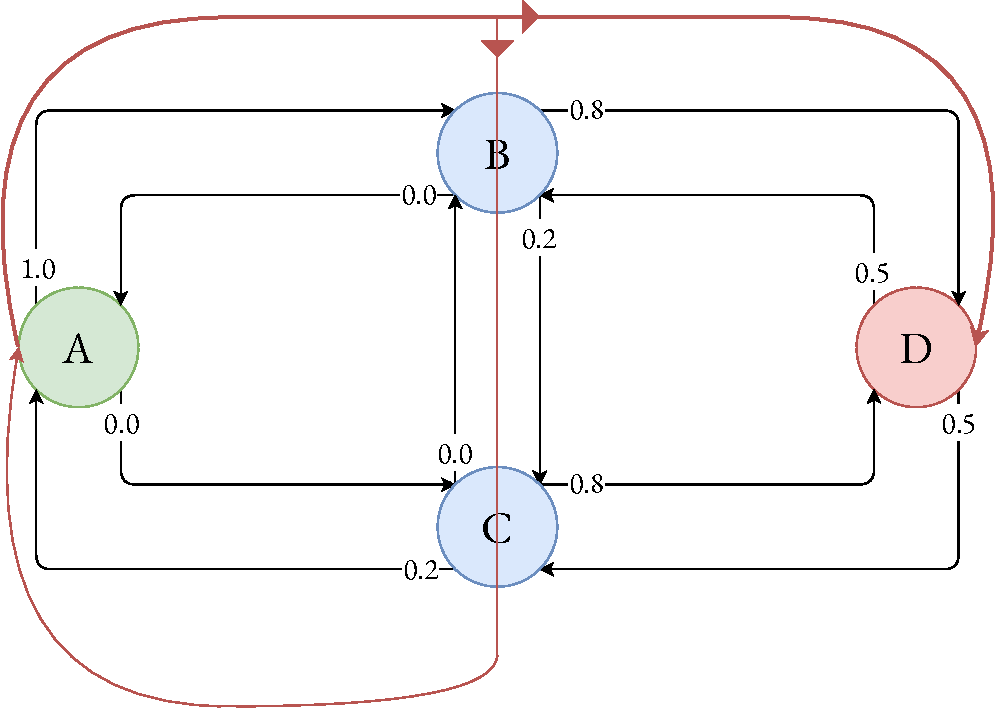
\includegraphics[width=0.8\textwidth]{figures/bad_route.pdf}
    \caption{An example of a bad routing created by the softmin routing strategy. A loop between nodes A, B, and C causes excess link utilisation and increased latency. The circles are vertices with A being the flow source and D the flow destination. The black lines are edges with the numbers signifying their splitting ratios. The red line is the flow induced by this particular routing.}
    \label{fig:bad_route}
\end{figure}


\todo{split pruning into separate section and writeup new alg}
\todo{cite DODAG and RLP and NP-hardness}
It can easily be seen that the problem of loops in the routing would not exist in a directed acyclic graph (DAG) as they are defined to have no cycles. Therefore, one way of avoiding routing loops is to convert the graph into a DAG by breaking links. A natural way to think about this is that for a path in a graph to be a cycle, it has to loop backwards on itself at some point. This means that at some point it is taking a step further away from the destination of the flow and back towards the source. As part of calculating the softmin routing we have already found the distance from each vertex to the destination. We can reuse this information to prune edges removing cycles. If, for every edge, we remove it if its head is further from the destination than its tail, then we know that traversing an edge can only ever bring us closer to the destination than we already are. If we remove all edges to more distant nodes then we have now created a DAG and so have no cycles. This method is also shown in algorithm~\ref{algorithm:softmin}.

\todo{write out the algorithm for softmin including pruning}
\begin{algorithm}[t]
\small
\begin{algorithmic}
\Function{GraphNetwork}{$E$, $V$, $\mathbf{u}$}
\EndFunction
\end{algorithmic}
\caption{Softmin routing algorithm: the steps taken to convert the learned edge weights given by the RL agent into a fully-defined routing strategy.}
\label{algorithm:softmin}
\end{algorithm}

\section{Traffic demand sequences}
We are using RL to approach this problem and the input to the agent is a history of previous demand matrices. The reason for this is that we have made the assumption that the sequence if DMs will have some sort of regularity which we can exploit to predict a routing strategy for the next timestep that is better than the optimal oblivious routing. Therefore, the demand sequences used for training such an agent must be built using some form of regularity. We try two different types of regularity heavily inspired by those selected by Valadrasky\cite{valadarsky2017learning}.

The first kind of regularity is \emph{cyclical}. Here we generate a cycle of demand matrices and the sequence is simply some number of repetitions of this cycle. The second kind is that of a \emph{gravity sequence}\cite{roughan2002experience}. This sequence again starts by defining a cycle which repeats but derives each subsequent DM as an averaging over the history rather than immediately presenting the next DM in the cycle. These scenarios make sense as temporal regularity is often seen in large networks such as those of ISPs\cite{fortz2002optimizing}. We also \emph{sparsify} the DMs (which consists of stochastically removing demands) to add noise to the regularity of the sequence.

\todo{Give mathematical definitions of DM sequences and sparsification}

The DMs in the cycles themselves are generated using a bimodal model\cite{medina2002traffic}. This is a model where demands are assigned randomly to flows, however, there is a small fixed probability that any such demand will be significantly larger than the rest (an elephant flow) which would impact the link utilisation if not handled carefully (thus aided by routing differently for different DMs).

\section{Training graphs}
For training and evaluation purposes it was important that the graphs trained on should be representative of real-world networks. It was thought that maybe graphs from this set could be generated. However, it is difficult to define the set of graphs akin to real-world AS networks. Fortunately, there is an open dataset, ``The Internet Topology Zoo''\cite{6027859} which contains a plethora of real-world networks, enough for both training and evaluation so it was decided to use this instead.
